\documentclass{iopart}

\usepackage{url}
\usepackage{amsbsy}
\usepackage{graphicx}

\newcommand{\eqref}[1]{{(\ref{#1})}}
\def\bSo{{\bf \hat{S}_1}}
\def\bSt{{\bf \hat{S}_2}}
\def\bL{{\bf \hat{L}_{N}}}
\def\hn{{\bf {\hat n}}}
 
\begin{document}

\title{The Mock LISA Data Challenges: from Challenge 1B to Challenge 3}

\author{The \emph{Mock LISA Data Challenge Task Force}:
Stanislav Babak$^\mathrm{aei}$,
John G. Baker$^\mathrm{gsfc}$,
Matthew J. Benacquista$^\mathrm{utb}$,
Neil J. Cornish$^\mathrm{montana}$,
Jeff Crowder$^\mathrm{jpl}$,
Shane L. Larson$^\mathrm{weber}$,
Eric Plagnol$^\mathrm{apc}$,
Edward K. Porter$^\mathrm{aei}$,
Michele Vallisneri$^\mathrm{jpl,cit}$,
Alberto Vecchio$^\mathrm{bgham,north}$
and the \emph{Challenge-1B participants}:
Keith Arnaud$^\mathrm{gsfc}$,
Leor Barack$^\mathrm{south}$,
Arkadiusz B{\l}aut$^\mathrm{wroclaw}$,
Curt Cutler$^\mathrm{jpl,cit}$,
Stephen Fairhurst$^\mathrm{cardiff}$,
Jonathan Gair$^\mathrm{cambridge,aei}$,
Xuefei Gong$^\mathrm{cas}$,
Ian Harry$^\mathrm{cardiff}$,
Deepak Khurana$^\mathrm{iit}$,
Andrzej Kr\'olak$^\mathrm{warsaw}$,
Ilya Mandel$^\mathrm{cit,north}$,
Reinhard Prix$^\mathrm{hannover}$,
B. S. Sathyaprakash$^\mathrm{cardiff}$,
Pavlin Savov$^\mathrm{cit}$,
Yu Shang$^\mathrm{cas}$,
Miquel Trias$^\mathrm{mallorca}$,
John Veitch$^\mathrm{bgham}$,
Yan Wang$^\mathrm{nanjing}$,
Linqing Wen$^\mathrm{aei,cit,uwa}$,
John T. Whelan$^\mathrm{aei}$}

\address{$^\mathrm{aei}$ Max-Planck-Institut f\"ur Gravitationsphysik (Albert-Einstein-Institut), Am M\"uhlenberg 1, D-14476 Golm bei Potsdam, Germany}
\address{$^\mathrm{apc}$ APC, UMR 7164, Univ.\ Paris 7 Denis Diderot, 10, rue Alice Domon et Leonie Duquet, 75025 Paris Cedex 13, France}
\address{$^\mathrm{bgham}$ School of Physics and Astronomy, Univ.\ of Birmingham, Edgbaston, Birmingham B152TT, UK}
\address{$^\mathrm{cambridge}$ Inst.\ of Astronomy, Univ.\ of Cambridge, Madingley Rd., Cambridge, CB30HA, UK}
\address{$^\mathrm{cardiff}$ School of Physics and Astronomy, Cardiff Univ., 5, The Parade, Cardiff, CF243YB, UK}
\address{$^\mathrm{cas}$ Inst.\ of Appl.\ Math, Acad.\ of Math.\ and System Sci., Chinese Academy of Sciences, 55 Zhongguancun Donglu, Beijing, 100080, China}
\address{$^\mathrm{cit}$ Theoretical Astrophysics, California Inst.\ of Technology, Pasadena, CA 91125}
\address{$^\mathrm{gsfc}$ Gravitational Astrophysics Lab., NASA Goddard Space Flight Center, 8800 Greenbelt Rd., Greenbelt, MD 20771, USA}
\address{$^\mathrm{hannover}$ Max-Planck-Institut f\"ur Gravitationsphysik (Albert-Einstein-Institut), D-30167 Hannover, Germany}
\address{$^\mathrm{iit}$ Indian Institute of Technology, Kharagpur, India}
\address{$^\mathrm{jpl}$ Jet Propulsion Laboratory, California Inst.\ of Technology, Pasadena, CA 91109, USA}
\address{$^\mathrm{mallorca}$ Dept. de F\'{\i}sica, Universitat de les Illes Balears, Cra. Valldemossa km. 7.5, E-07122 Palma de Mallorca, Spain}
\address{$^\mathrm{montana}$ Dept.\ of Physics, Montana State Univ., Bozeman, MT 59717, USA}
\address{$^\mathrm{nanjing}$ Dept.\ of Astronomy, Nanjing Univ., 22 Hankou Road, Nanjing, 210093, China}
\address{$^\mathrm{north}$ Dept.\ of Physics and Astronomy, Northwestern Univ., Evanston, IL, USA}
\address{$^\mathrm{south}$ School of Mathematics, Univ.\ of Southampton, Southampton, SO171BJ, UK}
\address{$^\mathrm{utb}$ Center for Gravitational Wave Astronomy, Univ.\ of Texas at Brownsville, Brownsville, TX 78520, USA}
\address{$^\mathrm{warsaw}$ Inst.\ of Mathematics, Polish Academy of Sciences, Warsaw, Poland}
\address{$^\mathrm{weber}$ Dept.\ of Physics, Weber State Univ., 2508 University Circle, Ogden, UT 84408, USA}
\address{$^\mathrm{wroclaw}$ Inst.\ of Theoretical Physics, Univ.\ of Wroc{\l}aw, Wroc{\l}aw, Poland}
\address{$^\mathrm{uwa}$ School of Physics, M013, Univ.\ of Western Australia, 35
Stirling Highway, Crawley, WA 6009, Australia}

\ead{Michele.Vallisneri@jpl.nasa.gov}

\begin{abstract}
The Mock LISA Data Challenges are a program to demonstrate LISA data-analysis capabilities and to encourage their development. Each round of challenges consists of several data sets containing simulated instrument noise and gravitational waves from sources of undisclosed parameters. Participants are asked to analyze the data sets and report the maximum information about the source parameters. The challenges are being released in rounds of increasing complexity and realism: here we present the results of Challenge 1B [issued... new groups...] and we describe Challenge 3 [which includes...].
\end{abstract}

\vspace{-18pt}
\pacs{04.80.Nn, 95.55.Ym}

% \maketitle

\section{Introduction}

Gravitational radiation from millions of sources, most of which in our Galaxy, but many populating the low-to-high redshift Universe, is expected to be recorded by the Laser Interferometer Space Antenna (LISA), an ESA/NASA mission to survey the gravitational wave (GW) sky in the frequency window $\sim 10^{-5}$--$10^{-1}$ Hz\cite{lisa}. Such variety of signals, overlapping in time and frequency space (to the limit of confusion in parts of the frequency range) poses a number of interesting new challenges in data analysis, whose solution is essential for the science exploitation of such a complex and innovative instrument.


%The Laser Interferometer Space Antenna (LISA), a NASA and ESA space mission to detect gravitational waves (GWs) in the $10^{-5}$--$10^{-1}$ Hz range \cite{lisa}, will produce time series consisting of the superposition of the signals from millions of sources, many in our Galaxy, some as far as the edge of the observable universe. Some of the signals, such as those from extreme--mass-ratio inspirals (EMRIs), are very complex functions of the source parameters; others, such as those from Galactic white-dwarf binaries, are simpler, but their resolution will be confused by the presence of many other similar signals that overlap in frequency space. Thus, data analysis is integral to the LISA measurement concept, because no source can be observed without first carefully teasing out its individual voice in the noisy party of the LISA data. Indeed, it is important to understand data analysis in order to demonstrate that LISA can meet its science requirements, and to translate these into decisions on instrument design.

The LISA International Science Team (LIST) initiated in 2005 a programme known as Mock LISA Data Challenges (MLDCs) with the goal of understanding at the conceptual and quantitative level the intricacies of LISA data analysis, of demonstrating LISA's observational capabilities and of beginning the development of data analysis algorithms, pipelines and prototype infrastructure: a Task Force chartered by the LIST issues periodically data sets containing synthetic noise and GW signals from sources of undisclosed parameters and challenge participants return detection candidates and parameter estimates that are then compared with those originally injected in the data sets.

%The idea of the Mock LISA Data Challenges (MLDCs) arose in late 2005 from this very realization. The MLDCs have the purpose of encouraging and tracking progress in LISA data-analysis development, and (as a useful byproduct) of producing a prototype of the LISA computational infrastructure, including common data formats, standard models of the LISA orbits, noises and measurements, software tools to generate waveforms and to simulate the LISA response, and more. The MLDCs are a coordinated (but voluntary) effort in the GW community, whereby a task force chartered by the LISA International Science Team periodically issues data sets containing synthetic noise and GW signals from sources of undisclosed parameters; challenge participants return detection candidates and parameter estimates, together with descriptions of their search methods. These results are then compiled and compared to the previously secret challenge ``key.'' \textbf{[These two paragraphs are verbatim from the MLDC-2 report. Need to rephrase, add news, more interesting comments.]}

Three rounds of MLDCs, spanning approximately six months each, have been completed so far. Challenge 1~\cite{mldclisasymp,mldcgwdaw1} focused on establishing the basic techniques to observe Galactic (intrinsically monochromatic) binaries, isolated or moderately interfering, and the in-spiral phase of bright, isolated non-spinning massive black hole (MBH) binary systems. Challenge 2~\cite{mldcgwdaw2} provided three considerably more complex subchallanges: a data set containing approximately 26 million (monochromatic) Galactic binaries drawn from a synthetic population; a data set with the same (though generated with different random seeds) Galactic binary population, with superimposed an unknown number (between 4 and 6) of in-spirals from nonspinning-MBH binaries with a range (between 10 and 2000) of single-interferometer optimal signal-to-noise ratios (SNRs) and coalescence times and five extreme-mass-ratio inspirals (EMRI) with optimal SNRs between 30 and 100. Lastly, five data sets each containing a single EMRI superimposed to Gaussian and stationary instrumental noise, with optimal SNRs between 40 and 110.

%Challenge 1, issued in Jun 2006 with results due in Dec 2006 (see \cite{mldclisasymp,mldcgwdaw1}), tackled the detection and parameter characterization of \emph{verification binaries} (Galactic binaries of known frequency and position); of loud unknown Galactic binaries, either alone or in small, moderately interfering groups; and of relatively loud inspirals of nonspinning supermassive--black-hole (MBH) binaries. All sources were represented by somewhat idealized waveforms, and they were staged on simulated instrument noise alone. Ten collaborations submitted entries, adopting a variety of methods (template-bank, stochastic- and genetic-optimization matched filtering; time--frequency; tomography; Hilbert transform). Despite the short timescale, each challenge was ``solved'' by at least one group, although some searches locked on strong secondary probability maxima for the source parameters. More important, Challenge 1 helped set the playing field and assemble the computational tools for the more realistic Challenge 2.

%Challenge 2, issued in Jan 2007 with results due at the end of Jun 2007, raised the bar by proposing three complex subchallenges. Data set 2.1 contained signals from a full population of Galactic binary systems (about 26 million sources). Data set 2.2 contained signals from a similar (but distinct) Galactic-binary population, plus an undisclosed number (between 4 and 6) of signals from nonspinning-MBH binary inspirals with optimal single-interferometer signal-to-noise ratios (SNRs) between 10 and 2000 and a variety of coalescence times, and plus five EMRI signals with optimal SNRs between 30 and 100. The EMRIs were modeled as Barack and Cutler's ``analytic kludges'' \cite{barackcutler}: adiabatic sequences of elliptical orbits emitting Peters--Mathews waveforms, with separation, precession and eccentricity evolving according to post-Newtonian equations. Last, five more data sets (denoted 1.3.1--5, since they were released at the time of Challenge 1) contained single EMRI signals over instrument noise alone, with optimal SNRs between 40 and 110. See \cite{mldcgwdaw2} for more details about the signal models and the ranges from which the source parameters were drawn.
%Altogether, Challenge 2 successfully demonstrated the identification of $\sim 20,000$ Galactic binaries, the accurate estimation of nonspinning-MBH inspiral parameters, and the positive detection of EMRIs.
%\textbf{[These two paragraphs are verbatim from the MLDC-2 report. Need to shorten, rephrase, add more about results.]}

The very steep increase in complexity introduced by Challenge 2 over a short time-scale and the need to consolidate analysis techniques before moving to even more taxing challenges motivated a second round of Challenge 1-type MLDCs. In particular, analysis pipelines for EMRIs, already included in Challenge 2, were particularly immature due to the complexity of the problem. These concepts inspired Challenge 1B, with data sets distributed in late Summer 2007 and results submitted in December 2007. Challenge 1B is in essence a fresh release of Challenge 1 data sets with the addition of data sets containing a single EMRI (with a range of SNRs) embedded in Gaussian and stationary instrumental noise. Ten collaborations took part to Challenge 1B. Highlights from this round include the range of techniques and groups that successfully recovered the signals from galactic binaries and MBH binary systems and the first convincing demonstration of the detection of EMRIs. An additional interesting though un-planned outcome of Challenge 1B was the lack of detection of any signal from a particular data set, where indeed gravitational waves were (unintentionally) generated with an SNR too low to allow their observation. Results from Challenge 1B are presented and discussed in Section~\ref{s:challenge-1b} and additional details are given in Refs XXX\textbf{[include GWDAW proceedings where available]}.

Challenge 3 data sets have just been released and results are due in December 2008. They introduce a number of innovations, including two new classes of signals -- short-lived bursts and isotropic stochastic backgrounds -- and more realistic galactic binary and MBH binary waveforms and LISA noise models. They also see for the first time the release of individual phase-meter channels for selected data sets. Section~\ref{s:challenge-3} is devoted to the descriptions of Challenge 3 innovations.


\section{Report on Challenge 1B}
\label{s:challenge-1b}

Challenge 1B focuses on three classes of sources treated independently: (monochromatic) galactic binaries, massive black hole binaries and extreme mass ratio inspirals. The results submitted by the participants were assessed still using the simple criteria considered in previous rounds~\cite{mldcgwdaw1, mldcamaldi2} whereby the parameters and waveform from the key file (corresponding to the true signal included in the data set) were compared to those recovered, using as figures of merit the {\em best recovered} SNR
%
\begin{equation}
\mathrm{SNR}_\mathrm{best}  = \frac{(A_\mathrm{true}|A_\mathrm{best}) + (E_\mathrm{true}|E_\mathrm{best})}
{\sqrt{(A_\mathrm{best}|A_\mathrm{best}) + (E_\mathrm{best}|E_\mathrm{best})}}\,,
\label{e:SNR}
\end{equation}
%
the {\em correlation}  
%
\begin{equation}
\label{cor}
C = \frac{\left(h_{\rm key}|h_{\rm rec}\right)}{\sqrt{\left(h_{\rm key}|h_{\rm key}\right)\left(h_{\rm rec}|h_{\rm rec}\right)}}\,,
\label{e:C}
\end{equation}
%
of the true waveform $h_{\rm key}$ with the recovered one $h_{\rm rec}$, and the simple difference 
%
\begin{equation}
\Delta\lambda = \lambda_{\rm key} - \lambda_{\rm rec}\,.
\label{e:deltalambda}
\end{equation}
%
between the true parameter in the key file $\lambda_{\rm key}$ and the "best fit" of the recovered parameter $h_{\rm rec}$. In the previous equations, $(.|.)$ stands for the usual inner product and $A$ and $E$ denote the two noise-orthogonal TDI channels.

\subsection{Galactic binaries: Challenges 1B.1.X}

Seven different Challenge 1B.1.X data sets contained signals from monochromatic binaries in a variety of combinations. Seven parameters are required to fully characterize each source: the amplitude $\mathcal{A}$, the (constant) frequency $f$, the sky location $\theta,~\phi$, the inclination angle $\iota$, the polarization angle $\psi$, and the initial phase $\phi_0$. Five groups -- members of the Goddard Space Flight Center (GSFC), a group from the Institute of Mathematics of the Polish Academy of Science and the Institute of Theoretical Physics at the University of Wroclaw (IMPAN), members of the Max Planck Institute for Gravitational Physics, the Albert Einstein Institute (AEI), a collaboration of scientists from the Institute of Applied Mathematics of the Chinese Academy of Sciences and the Department of Astronomy of Nanjing University (MCMNJU) and members of the Universitat de les Illes Balears and the University of Birmingham (UIBBham) --   submitted entries for this class of Challenges, though many groups concentrated only on  selected data sets and only AEI provided entries for every challenge. 

A fair range of techniques was considered. They broadly belong to the same classes adopted in the past for similar MLDCs, see Refs.~\cite{mldcgwdaw1, mldcamaldi2} and references therein. An healthy spectrum of techniques has therefore been identified and has begun to consolidate for this class of signals, but new implementations and different technical solutions are being pursued. GSFC used the X-Ray Spectral Fitting Package (XSPEC)~\cite{XSPEC_website} to fit templates to the energy spectra. The package includes a Levenberg-Marquardt optimization algorithm which was used to obtain an initial guess for the source parameters. A Markov Chain Monte Carlo (MCMC) routine, also available in XSPEC, was then used to arrive at the best fit parameters for the sources. IMPAN used a grid-based search featuring a constraint optimal hypercube lattice and matched filtering; the ${\cal F}$-statistic~\cite{fstat} was employed to reduced the search space from $7$ to $3$ parameters. A similar technique was adopted by AEI, and a more complete description of the method is found in~\cite{prixwhelan}, though the current modeling of the waveform has been updated to the rigid adiabatic approximation instead of using the long-wavelength limit. MCMNJU, used a genetic algorithm featuring the ${\cal F}$-statistic to determine the source parameters, and UIBBham used a MCMC approach, described in more detail in~\cite{tvv}.

%There were four collaborations that participated in the searches of the MLDC data sets containing monochromatic sources. The participants from the Goddard Space Flight Center (GSFC) used the X-Ray Spectral Fitting Package (XSPEC)~\cite{XSPEC_website} to fit templates to the energy spectra. The package includes a Levenberg-Marquardt optimization algorithm which was used to get an initial guess for the source parameters. A Markov Chain Monte Carlo (MCMC) routine, also available in XSPEC, was then used to arrive at the best fit parameters for the sources. The collaboration from the Institute of Mathematics of the Polish Academy of Science (IMPAN) and the Institute of Theoretical Physics at the University of Wroclaw, performed a grid-based search featuring a constraint optimal hypercube lattice and matched filtering. They also use the ${\cal F}$-statistic~\cite{fstat} to shrink the search space from $7$ to $3$ parameters. The participants from the Max Planck Institute for Gravitational Physics, the Albert Einstein Institute (AEI), also used a grid-based approach using the ${\cal F}$-statistic. A more complete description of the method is found in \cite{AEI_MLDC_1_paper}, though the current modeling of the waveform has been updated to the rigid adiabatic approximation instead of using the long-wavelength limit. A collaboration of people from the Institute of Applied Mathematics of the Chinese Academy of Sciences and the Department of Astronomy of Nanjing University (MCMNJU), used a genetic algorithm featuring the ${\cal F}$-statistic to determine the source parameters.


%For monochromatic white dwarf--white dwarf (WDWD) binary systems seven parameters are required to fully characterize each source. These parameters are the amplitude $\mathcal{A}$, the frequency $f$, the sky location $\theta,~\phi$, the inclination angle $\iota$, the polarization angle $\psi$, and the initial phase $\phi_0$. 


Three data sets, Challenges 1B.1.1a-c, contained a single monochromatic binary -- the main difference between the data sets was the source's frequency -- with SNR $\approx 13-25$. Table~\ref{Table_1b_1_1_correlations} summarises the values of the correlations, see Eq.~(\ref{e:C}) for each challenge entry. As some of the entries had close fits to the intrinsic parameters ($f$, $\theta$, and $\phi$), but had issues matching the remaining (extrinsic) parameters, these parameters were recalculated using the ${\cal F}$-statistic~\cite{fstat}. Results for these recalculated parameters are also provided. Table~\ref{Table_1b_1_1_parameter_differences} provides the deviations of the parameter values from the values in the key files of Challenges 1B.1.1a-c. Figure~\ref{Figure_1b_1_1a_sky_positions} shows how the various groups succeeded in extracting the sky position of the source in Challenge 1b.1.1a.

\begin{figure}
\centerline{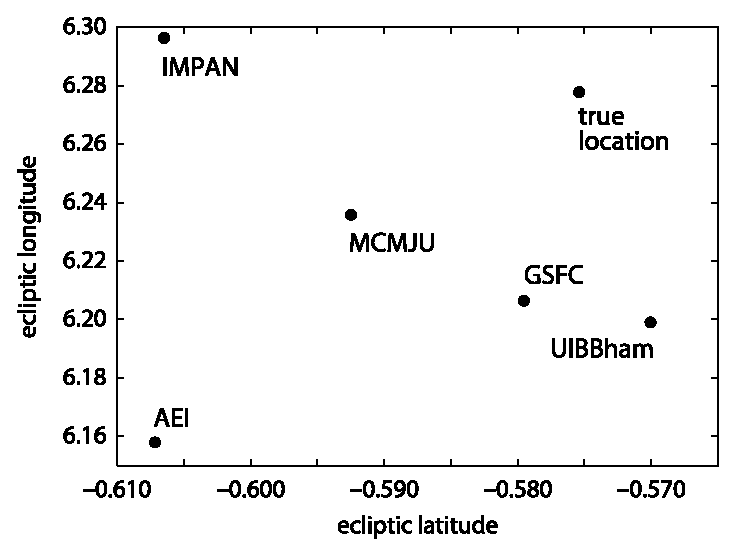
\includegraphics[width=7.5cm]{MLDC_1b-1.1a_sky_positions.eps}}
\caption{Plot of the sky position for the source from the key file, for Challenge 1b.1.1a, and the recovered sky position for each of the entries.\label{Figure_1b_1_1a_sky_positions}}
\end{figure} 

\begin{table}
\caption{\label{Table_1b_1_1_correlations} The performance of challenge entries on the single galactic binary challenges as calculated using SNR, and $C$. Data in which the extrinsic parameters were corrected using the ${\cal F}$-statistic are denoted with an asterisk (*); numbers are not reported where the frequency is well off, and the $\mathcal{F}$-statistic is only fitting to noise.}
\begin{indented}
\item[]\begin{tabular}{lrrrrrr}
\br
Group & SNR & $C$ & SNR & $C$ & SNR & $C$ \\
\br
& \centre{2}{Challenge 1b.1.1a}
& \centre{2}{Challenge 1b.1.1b}
& \centre{2}{Challenge 1b.1.1c} \\
& \centre{2}{(${\rm SNR}_{\rm key}=13.819$)}
& \centre{2}{(${\rm SNR}_{\rm key}=24.629$)}
& \centre{2}{(${\rm SNR}_{\rm key}=15.237$)} \\
\mr
AEI			& 20.435	& 0.108	& 18.652	& 0.922 & 1.949	& -0.190		\\
AEI*			& 14.199	& 0.984	& 23.266	& 0.996	& 14.770	& 0.989 \\
GSFC			& 13.805	& 0.992	& 20.310	& 0.807	& 4.827		& -0.138\\
GSFC*		&       &     	& 20.987	& 0.814 \\
IMPAN		& 14.427	& 0.988	& 25.235	& 0.981 & 16.465	& 0.925	\\
IMPAN*		&       &     	& 23.152	& 0.997 & 14.194	& 0.946	\\
MCMNJU			& 13.524	& 0.952	& 22.641	& 0.906	& 6.830	& 0.033 \\
MCMNJU*			& 14.193	& 0.996	& 23.270	& 0.994	\\
UIBBham			& 13.577	& 0.992	& 23.479	& 0.996 	\\
\br
\end{tabular}
\end{indented}
\end{table}

\begin{table}
\caption{\label{Table_1b_1_1_parameter_differences} The performance of challenge entries on the single galactic binary challenges as calculated using recovered parameter differences. Data in which the extrinsic parameters were corrected using the ${\cal F}$-statistic are denoted with an asterisk (*).}
\begin{indented}
\item[]\begin{tabular}{lrrrrrrr}
\br
Group & $\Delta \theta$ & $\Delta \phi$ & $\Delta f$ (nHz) & $\Delta\psi$ & $\Delta \iota$ & $\Delta \varphi$ & $\Delta \mathcal{A} (\times 10^{-23})$ \\
\br
\centre{8}{Challenge 1b.1.1a} \\
\mr
AEI		& 0.0318	& -0.120	& -2.43		& 0.217		& -0.454 	& 1.17		& 1.22		\\
AEI*		& 0.0318	& -0.120	& -2.43		& 0.700		& 0.215		& -1.23		& 1.18		\\
GSFC		& 0.00412	& -0.0715	& -1.81	 	& 0.708	 	& 0.252 	& 1.33	 	& 1.20		\\
IMPAN		& 0.0311	& 0.0185 	& 2.13		& 0.454 	& 0.212	 	& -1.06 	& 1.25		\\ 
MCMNJU		& 0.0170	& -0.0424	& -0.534	& 0.662		& 0.426		& -1.57		& 2.34		\\
MCMNJU*		& 0.0170	& -0.0424	& -0.534	& 0.746		& 0.248		& -1.44		& 1.37		\\
UIBBham		& -0.00540	& -0.0790	& -1.51		& 0.708		& 0.173		& -1.32		& 0.647		\\
\br
\centre{8}{Challenge 1b.1.1b} \\
\mr
AEI		& 0.0558	& -0.00899	& 0.946		& -1.05		& 0.283		& 1.63		& -0.0664	\\
AEI*		& 0.0558	& -0.00899	& 0.946		& -0.761	& 0.0776	& 1.46		& 0.00307	\\
GSFC		& 0.462		& 0.0606	& -30.9		& 2.56		& 0.182		& 0.516		& -0.0245	\\
GSFC*		& 0.462		& 0.0606	& -30.9		& -0.534	& 0.198		& 0.624		& 0.0665	\\
IMPAN		& -0.0203 	& 0.000708	& 0.852 	& 0.333 	& 0.339 	& -0.603 	& 0.713		\\ 
MCMNJU		& 0.0670	& -0.00627	& 2.069530	& -0.732	& -0.0643	& 0.844		& -0.223	\\
MCMNJU*		& 0.0670	& -0.00627	& 2.069530	& -0.739	& 0.0633	& 1.30		& -0.0165	\\
UIBBham		& 0.0436	& -0.00817	& 1.777530	& -0.636	& 0.0428	& 1.13		& -0.0293	\\
\br
\centre{8}{Challenge 1b.1.1c} \\
\mr
AEI		& 0.0261	& 0.00530	& 1.84		& -0.499	& -1.12		& 3.02		& 0.124		\\ 
AEI*		& 0.0261	& 0.00530	& 1.84		& 0.0410	& -0.0937	& -0.123	& 0.106		\\ 
GSFC		& 0.452		& -1.48		& 140		& 1.82		& -0.471	& -0.663	& -0.695	\\ 
IMPAN		& 0.0158	& 0.0248	& 3.72		& -1.51		& -0.197	& 2.68		& 0.478		\\ 
IMPAN*		& 0.0158	& 0.0248	& 3.72		& -0.0287	& -0.113	& 0.356		& 0.0792	\\ 
MCMNJU		& 0.555		& -0.368	& 359		& -1.59		& -0.250	& -0.943	& -0.532	\\ 
\br
\end{tabular}
\end{indented}
\end{table}

The Challenge 1b.1.2 data set contained 25 ``verification'' binaries, defined as sources for which frequency and sky location are exactly known. This simulates the search for signals from galactic binaries that are already known to exist. In fact, five of these binaries are taken from a list of known binaries available on Gijs Nelemans' website~\cite{nelemanswiki}, while the remaining twenty were simulated binaries. Table~\ref{Table_1b_1_2_correlations} contains the global SNRs and correlations between all sources characterized by the parameters in the key file and the sources recovered by the three groups that participated in this challenge. As in Challenges 1B.1.1a-c the issue with the extrinsic parameters caused the correlations to be less than ideal. However, as the intrinsic parameters were provided to the participants an ${\cal F}$-statistic calculations were not performed. 

\begin{table}
\caption{\label{Table_1b_1_2_correlations} The performance of challenge entries on the verification binaries challenge as calculated using SNR, and $C$.}
\begin{indented}
\item[]\begin{tabular}{lrrc}
\br
Group & SNR & $C$ & \# Recovered\\
\br
\centre{4}{Challenge 1b.1.2 (${\rm SNR}_{\rm key}=634.918$, $25$ Sources)}  \\
\mr
AEI		& 891.677	& -0.822	& 25	 	\\
GSFC		& 807.012	& 0.006		& 25	 	\\
MCMNJU		& 603.805	& 0.267		& 25	 	\\
\end{tabular}
\end{indented}
\end{table}

The data set for Challenge 1b.1.3 contained the signals from $20$ unknown binaries distributed across the LISA band and therefore well separated in frequency space. Unfortunately, there was an issue with the generation of the signals that caused their SNRs to be too small for detection (all were below $1$). As a silver lining to this cloud, none of the participating groups responding to this challenge reported a positive detection, providing therefore a meaningful consistency test of the performance of the algorithms.

Challenge 1b.1.4 was a test of the search algorithms in the presence of mild source confusion. Fifty-one sources were spread across a $15 \mu{\rm Hz}$ band starting at $3\, {\rm mHz}$, with an average source density of 0.108 sources per frequency bin. Challenge 1b.1.5 tested the algorithms in the presence of a higher level of source confusion, comparable to that actually produced by our Galaxy during the LISA mission: forty-four sources were spread across a $3 \mu{\rm Hz}$ band centered on $3 {\rm mHz}$; a source density of 0.465 sources per frequency bin. The presence of multiple sources in the data streams of these challenges introduces the possibility of the search algorithms missing sources (false negatives) as well as returning detections when no source is actually present (false positives). To determine the presence of false positives we first matched the frequencies of the recovered sources and those from the key file to within one frequency bin (${1}/{{\rm year}}$) of each other. If the correlation between the pair was less than 0.7 (after correcting with the ${\cal F}$-statistic) the recovered source was considered a false positive. The two measures for the matches in these challenges, as in Challenge 1B.1.2, are the SNR and correlation. Again, we use the combined signal from all recovered sources compared to the signal from the sources in the key file. Tables~\ref{Table_1b_1_4_correlations} and~\ref{Table_1b_1_5_correlations} give the results of the two entries to Challenge 1b.1.4 and the single entry to Challenge 1B.1.5. Figure~\ref{Figure_1b_1_4_AEI} shows plots the MLDC signal from the sources in Challenge 1B.1.4 and the residuals after subtracting the signal from the sources entered by the AEI, before and after the ${\cal F}$-statistic correction.

\begin{figure}
\centerline{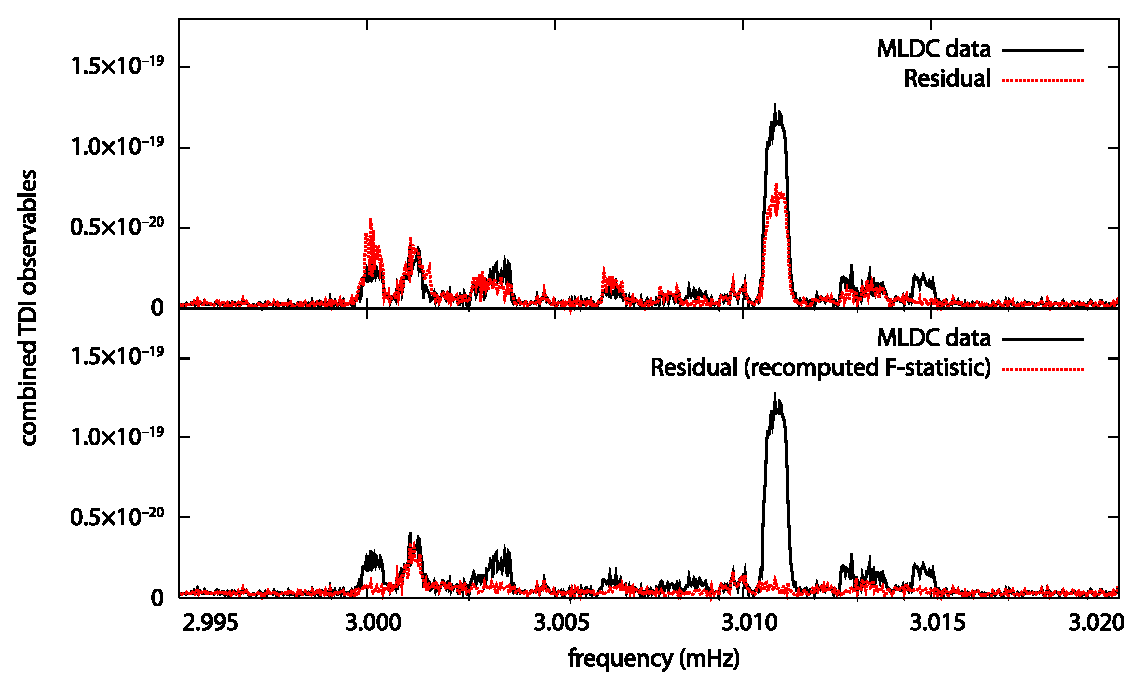
\includegraphics[width=10cm]{MLDC_1b-1.4_AEI_comb.eps}}
\caption{\label{Figure_1b_1_4_AEI}Plot of the amplitude of the signal in MLDC 1b.1.4 and the residual after subtracting the signal from the AEI entry, before and after the ${\cal F}$-statistic correction.}
\end{figure} 

\begin{table}
\caption{\label{Table_1b_1_4_correlations} The performance of challenge entries on the mildly confused binaries challenge as calculated using SNR, and $C$. Data in which the extrinsic parameters were corrected using the ${\cal F}$-statistic are denoted with an asterisk (*).}
\begin{indented}
\item[]\begin{tabular}{lrrcc}
\br
Group & SNR & $C$ & \# Recovered & False Positives \\
\br
\centre{5}{Challenge 1b.1.4 (${\rm SNR}_{\rm key}=340.233$, $51$ Sources)}  \\
\mr
AEI		& 375.366	& 0.774		& 13	& 2	\\
AEI*		& 329.344	& 0.966		& 13	& 2	\\
GSFC		& 209.411	& 0.003		& 6	& 1	\\
GSFC*		& 90.506	& 0.282		& 6	& 1	\\
\end{tabular}
\end{indented}
\end{table}

\begin{table}
\caption{\label{Table_1b_1_5_correlations} The performance of challenge entries on the highly confused binaries challenge as calculated using SNR, and $C$. Data in which the extrinsic parameters were corrected using the ${\cal F}$-statistic are denoted with an asterisk (*).}
\begin{indented}
\item[]\begin{tabular}{lrrcc}
\br
Group & SNR & $C$ & \# Recovered & False Positives\\
\br
\centre{5}{Challenge 1b.1.5 (${\rm SNR}_{\rm key}=273.206$, $44$ Sources)}  \\
\mr
AEI		& 208.273	& 0.453		& 3	 & 0	\\
AEI*		& 251.985	& 0.929		& 3	 & 0	\\
\end{tabular}
\end{indented}
\end{table}

\subsection{Massive Black Hole Binary Systems: Challenges 1B.2.X}

Two data sets were released each containing a single and loud in-spiral signal from a MHB binary embedded in Gaussian and stationary noise; as in all the challenges so far, the in-spiral waveform was approximated the restricted post$^2$-Newtonian order and the black holes are assumed to be non-spinning and in a circular orbit (see Section~\ref{s:challenge-3} for the important difference in the waveform model introduced starting from Challenge 3). Nine parameters described the waveform: the two masses $m_{1,2}$, the time to coalescence of the binary $t_c$, the sky position $(\beta,\lambda)$, the luminosity distance $D_L$, the orbital inclination angle $\iota$, the gravitational polarization angle $\psi$ and the initial gravitational wave phase $\varphi_0$.  The prior range, known to the Challenge participants, from which the signals were drawn was The groups were given the following limited prior information on the parameters of the systems.  One of the individual masses in each case would be in the range $1\leq m_1/10^6\,M_{\odot}\leq 5$, while the other mass would be in the range $m_2=m_1/x$ where $1\leq x\leq 4$.  The time to coalescence  would be $t_c = 6\pm 1$ months for Challenge 2.1 and $t_c=400\pm40$ days for Challenge 2.2.\\


\noindent Two groups submitted results for the massive black hole search :\\

\noindent\emph{ JPL} : used a three step strategy combining a time-frequency track search analysis, followed by a template bank matched filter search, finishing with a Metropolis-Hastings Monte Carlo refinement.  The JPL group submitted entries for both 2.1 and 2.2.\\
\emph{ Cardiff} : used a stochastic template bank matched filter search\cite{cardiffmbh}.  The Cardiff group submitted an entry for 2.1.\\

We can see from Table~\ref{mbh} that both groups did well in recovering the parameters of the injected binary systems.  In all cases the groups recovered almost all of the combined key SNR: the key values were 531.84 and 80.67 for 1B.2.1 and 1B.2.2 respectively.  For challenge 1B.2.1, JPL recovered an SNR of 531.57, while Cardiff recovered an SNR of 511.78.  In challenge 1B.2.2, JPL recovered an SNR of 79.86.  In the table we have adjusted the error estimates for degeneracies when certain symmetries are taken into account.  In challenge 1B.2.1, for both JPL and Cardiff, the error values for the polarization angle are given using the symmetry $\psi\rightarrow\psi+2\pi$.  In challenge 1B.2.2, the error values for both $\psi$ and $\varphi_0$ in the JPL entry are due to the symmetries $\psi\rightarrow\psi+\pi/2$ and $\varphi_0\rightarrow\varphi_0-\pi$.  

It is interesting to note that in challenge 1B.2.1, both JPL and Cardiff ended up on secondary sky positions that affected the precision of the other extracted parameters.  In fact the JPL entry is almost at the antipodal sky position, which explains the large errors in $\beta$ and $\lambda$, while still recovering almost the full SNR.  This result is a continuing reminder of a role that the antipodal sky solutions play for the extraction of MBHs from the LISA data stream.  It is clear after the three challenges to date,  for MBHs, it is always safer to try and return two sky solutions for recovered parameters.  In the real LISA case, because of the symmetric sensitivity of the beam pattern functions, we will be unable to distinguish between the two sky solutions a priori.

\begin{table}
\caption{\label{mbh}Relative/absolute errors for the MBH binaries recovered by the JPL and Cardiff groups in Challenges 1B.2.1 and 1B.2.2.}
\begin{indented}\lineup
\item[]\begin{tabular}{@{}llll}
\br
Challenge          & \multicolumn{2}{c}{1B.2.1} & \multicolumn{1}{c}{1B.2.2} \\
${\rm SNR}_{\rm key}$        & \multicolumn{2}{c}{531.84}	&	\multicolumn{1}{c}{80.67} \\
\mr
Group          & \multicolumn{1}{c}{JPL} & \multicolumn{1}{c}{Cardiff} & \multicolumn{1}{c}{JPL} \\
\mr
${\rm SNR}$ 	& \multicolumn{1}{c}{531.57}	&	\multicolumn{1}{c}{511.78}	&	\multicolumn{1}{c}{79.86}	\\
$\Delta m_{1}/m_{1}$  & \m$5.991 \times10^{-3}$   & \m0.108    & \m0.122\\
$\Delta m_{2}/ m_{2}$ & $-5.252 \times10^{-3}$    & $-0.111$    & $-0.134$\\
$\Delta t_c/ t_c$     & \m$1.369\times10^{-5}$  & $-3.601\times10^{-5}$ & $-7.296\times10^{-5}$\\
$\Delta D_L/ D_L$     & $-0.139$                    & $-1.438$         & \m$4.781\times10^{-3}$\\
$\Delta \beta$        & \m2.429                   & \m1.374         & \m$5.862\times10^{-3}$\\
$\Delta \lambda$      & \m3.133                   & \m0.548          & $-1.461\times10^{-2}$\\
$\Delta \iota$        & \m0.713                   & \m0.678         & $-6.955\times10^{-2}$\\
$\Delta \psi$         &$-0.564$                     & \m1.448 & $-4.878\times10^{-2}$\\
$\Delta \varphi_0$    &$-2.846$                    & $-2.389$        & $-1.584$\\
\br
\end{tabular}
\end{indented}
\end{table}

\subsection{Challenges 1B.3.X: EMRIs}

Three groups participated in this challenge and those are the same groups which 
submitted results for the challenge 2 \cite{mldcgwdaw2}. The basic underlying techniques 
used in the extracting the parameters remained the same, but were further 
improved and tuned (see more detailed article on EMRIs in this issue).
The challenge for EMRIs had five data sets with a single signal in each, for details on the 
parameter distribution and SNRs we refer reader to \cite{mldcgwdaw2}. The evaluation of the 
results was performed along the same line as for the challenge 2 and similar to the MBH binaries 
evaluation. In particular we have computed overlaps of the signals generated with recovered 
parameters with the true signal for each $A$ and $E$ channels. We have also evaluated 
combined SNR between the data set and the recovered signal (see Table~\ref{EMRI1}).
 For the results submitted by Gair, Mandel, and Wen (EtfAG, \cite{gmw}) we could not evaluate overlaps and 
 SNR since their method (based on the time-frequency analysis) targeted only intrinsic parameters and was insensitive to the initial phases. Therefore we have produced also the table of the relative errors in the parameter estimation and the results are summarized in the 
 Table~\ref{EMRI2}.
 
 \begin{table}
\caption{\label{EMRI1} Errors for challenge 1.3.X}
\begin{tabular}{|c|c|c|c|c|c|c|c|c|c|c|c|c|c|c|}
\hline
Entry &  $\frac{d\beta}{\Delta\beta}$ & 
$\frac{d\lambda}{\Delta\lambda}$ &
 $\frac{d\theta_K}{\Delta\theta_K}$ & $\frac{d\phi_K}{\Delta\phi_K}$ 
 & $\frac{da}{\Delta a}$ & $\frac{d\mu}{\Delta\mu}$ & 
 $\frac{dM}{\Delta M}$ &  $\frac{d\nu_0}{\nu_0}$ 
  &  $\frac{de_0}{0.15}$  & 
 $\frac{d\lambda_{SL}}{\Delta\lambda_{SL}}$ \\ 
\hline
BBGP-1B.3.1 & -0.03   &   -0.0059   &   -0.14   &   0.053   &   0.31   &   -0.20   &   -0.84   &   0.026    &   0.37     &   -0.022   \\
EtfAG-1B.3.1  & 0.019   &   -0.0045   &   0.56   &   0.33   &   0.16   &   -0.11   &   -0.27   &   -9.3e-05    &   0.17     &   0.078    \\
MT2-1B.3.1  &  0.0058   &   0.0027   &   0.00044   &   0.0051   &   -0.0022   &   0.0065   &   0.014   &   3.2e-06      &   -0.0085    &   -0.0020   \\
\hline
BBGP-1B.3.2  &  -0.16   &   -0.43   &   0.46   &   -0.33   &   -0.0088   &   -0.0040   &   0.016   &   0.00014     &   -0.010    &   -0.0013   \\
EtfAG-1B.3.2  &  -0.014   &   0.0042   &   0.97   &   -0.36   &   0.0043   &   -0.046   &   -0.069   &   -6.5e-05     &   0.041     &   0.0041  \\
MT2-1B.3.2  & 0.0040   &   -0.0086   &   0.79   &   0.41   &   0.093   &   -0.064   &   0.35   &   -0.035    &   0.068    &   0.092    \\
\hline
BBGP-1B.3.3 &   0.091   &   0.50   &   -0.23   &   0.045   &   -0.32   &   -0.49   &   -0.029   &   0.00061      &   0.019     &   0.054   \\
EtfAG-1B.3.3  &  -0.01   &   -0.004   &   0.49   &   -0.34   &   0.0073   &   -0.059   &   -0.061   &   -7.8e-05    &   0.038      &   0.0061  \\
MT2-1B.3.3  &  0.045   &   -0.019   &   -0.1   &   0.077   &   -0.066   &   0.13   &   0.59   &   0.00036   &   -0.33     &   0.010  \\
\hline
BBGP-1B.3.4 &  -0.57   &   -0.37   &   0.37   &   -0.31   &   -0.025   &   0.020   &   -0.88   &   0.066     &   0.065     &   -0.16   \\
EtfAG-1B.3.4 & -0.56   &   0.49   &   0.56   &   -0.34   &   0.059   &   0.12   &   0.04   &   0.00028    &   -0.039    &   0.0040   \\
\hline
BBGP-1B.3.5 &  -0.48   &   -0.14   &   -0.35   &   0.1   &   -0.094   &   -0.094   &   0.55   &   -0.0021    &   -0.017      &   -0.060  \\
EtfAG-1B.3.5 &  -0.58   &   0.46   &   0.27   &   -0.084   &   0.20   &   -0.7   &   0.83   &   -0.066     &   0.066     &   0.27  \\
\hline
\end{tabular}
\end{table}

\begin{table}
\caption{\label{EMRI2} Overlaps for challenge 1.3.X, the true SNR are: 1.3.1 - 123.7, 1.3.2 - 133.46, 1.3.3 - 81.0, 1.3.4 - 104.5, 1.3.5 - 57.6.} 
\begin{tabular}{|c|c|c|c|c|c|}
\hline
Entry & overlap (A) & $SNR_A$ &  overlap (E) & $SNR_E$ & $SNR$ \\
\hline
BBGP-1B.3.1 & 0.57 & 51 .0 & 0.58 & 51.6 & 72.5\\
MT2-1B.3.1  & 0.998 & 86.1 & 0.997 & 88.3 & 123.4\\
\hline
BBGP-1B.3.2 & 0.07 & 6.6 & 0.18 & 18.2 & 17.6\\
BBGP-1B.3.2$^\mathrm{a}$ & 0.39 & 37.6 & 0.41 & 39.8 & 54.7\\
MT2-1B.3.2  & 0.54 & 49.5 & 0.54 & 50.8 & 70.9 \\
\hline
BBGP-1B.3.3 & -0.06 & -4.2 & -0.0003 & -0.05 & -3.0 \\
BBGP-1B.3.3$^\mathrm{a}$ & -0.2 & -11.5 & -0.32 & -19.0 & -21.5\\
MT2-1B.3.3  & 22.0 &  22.0 & 20.5 & 20.9 & 30.4 \\
\hline
BBGP-1B.3.4 & 0.0007 & 2.1 & -0.0002 & 0.8 & 2.1\\
BBGP-1B.3.4$^\mathrm{b}$ & 0.16 & 13.9 & 0.04 & 6.7 & 14.6 \\ 
\hline
BBGP-1B.3.5 & 0.09 & 3.4 & 0.1 & 4.2 & 5.3\\
\hline
\end{tabular}\\
$^\mathrm{a}$ corrected sign of the latitude\\
$^\mathrm{b}$ corrected phases at $t=0$
\end{table}


From booth tables one can see clear detection and excellent estimation of the parameters for
1.3.1 by MT2 group (N. Cornish). Other submissions seem to suffer by the same problem as before (in challenge 1): the search algorithm got stack at the secondary maxima. 
 



\section{Synopsis of Challenge 3}
\label{s:challenge-3}

The third round of the MLDCs consists of five challenges (3.1--3.5):
%
\begin{itemize}
%
\item \textit{Data set 3.1} contains a Galactic GW foreground from $\sim$ 60 million compact binary systems.
This data set is a direct descendant of Challenge 2.1, but it improves on the realism of the latter by including both detached and interacting binaries with intrinsic frequency drifts (either positive or negative). Section \ref{sec:ch3galaxy} gives details about the binary waveform models, about their implementation in the LISAtools codebase, and about the generation of the Galactic population. 
%
\item \textit{Data set 3.2} contains GW signals from 4--6 binaries of spinning massive black holes (MBHs), on top of a confusion Galactic-binary background. This data set improves on the realism of Challenges 1.2.1--2 and 2.2 by modeling the orbital precession (and ensuing GW modulations) due to spin--orbit and spin--spin interactions. Section \ref{sec:ch3mbh} gives details about the MBH-binary waveforms.

Because this challenge focuses on the effects of spins rather than on the joint search for MBH signals and for the brightest Galactic binaries, the background is already \emph{partially subtracted}---it is generated from the population of detached binaries used for Challenge 3.1, withholding all signals with SNR $> 5$.
%
\item \textit{Data set 3.3} contains five GW signals from extreme--mass-ratio inspirals (EMRIs). As in Challenges 1.3.1--5, EMRI waveforms are modeled with Barack and Cutler's ``analytic kludge'' waveforms \cite{barackcutler}; this challenge introduces the complication of detecting five such signals with lower SNRs, and \emph{in the same data set}. By contrast, Galactic confusion is not included. See section \ref{sec:ch3emri} for details.
%
\end{itemize}
%
Data sets 3.1--3 consist of approximately two years of data ($2^{22}$ samples at a cadence of $15$ s) for time-delay interferometry (TDI) observables $X$, $Y$, and $Z$. These data sets are released both as time series of equivalent strain generated by the LISA Simulator \cite{lisasimulator} and as time series of fractional frequency fluctuations generated by Synthetic LISA \cite{synthlisa}; see \cite[p.\ S556]{mldcgwdaw2} for the conversion between the two. Indeed (with a few exceptions, described below, for 3.4 and 3.5), the Challenge-3 data sets are built using the ``pseudo-LISA'' model of Challenges 1 and 2: the orbits of the LISA spacecraft are $e^2$-accurate Keplerian ellipses with conventional orientations and time offsets; \emph{modified} TDI (a.k.a.\ TDI 1.5) expressions are used for the observables; and Gaussian, stationary instrument noise is included from six proof masses and six optical benches with known noise levels that are identical across each set of six.\footnote{The six proof-mass noises are uncorrelated and white in acceleration, with one-sided power spectral density (PSD)
%
\begin{displaymath}
S_\mathrm{acc}^{1/2}(f) = 3 \times 10^{-15} [1 + (10^{-4}\,{\rm Hz}/f)^2]^{1/2} \, \mathrm{m}\, \mathrm{s}^{-2}\, \mathrm{Hz}^{-1/2};
\end{displaymath}
%
the six optical-path noises are uncorrelated and white in phase with with PSD
%
\begin{displaymath}
S_\mathrm{opt}^{1/2}(f) = 20 \times 10^{-12} \, \mathrm{m}\, \mathrm{Hz}^{-1/2};
\end{displaymath}
%
\textbf{[Neil: insert conversion to LISA Simulator values?]}
the conversion to Synthetic LISA's dimensionless fractional frequency fluctuations is described on \cite[p.\ 6]{synthlisa}; the values actually used in the MLDCs are
%
\begin{displaymath}
S_\mathrm{acc}(f) = 2.5 \times 10^{-48} (f/\mathrm{Hz})^{-2} [1 + (10^{-4}\,{\rm Hz}/f)^2] \, \mathrm{Hz}^{-1};
\end{displaymath}
\begin{displaymath}
S_\mathrm{opt}(f) = 1.8 \times 10^{-37} (f/\mathrm{Hz})^{2} \, \mathrm{Hz}^{-1}.
\end{displaymath}
} See \cite{mldcgwdaw2} for details.

Challenges 3.4 and 3.5 address the detection of two GW sources that are \emph{new} to the MLDCs, and that have (respectively) bursty and stochastic characters: thus, these searches require an accurate characterization of instrument noise, which in reality will not be available \emph{a priori}, but will be obtained from the LISA measurements themselves.
To model this problem, in data sets 3.4 and 3.5 the levels of the six + six secondary noises have been independently randomized by $\pm 20 \%$ (the noises are however still uncorrelated). In addition, these data sets contain time series for all twelve ``raw'' LISA phase measurements $y_{ijk}$ and $z_{ijk}$ \cite{synthlisa}, so that contestants may now build additional TDI observables to help characterize instrument noise. The phase measurements \emph{do} include laser phase noise, because otherwise they would convey extra information unavailable from the real LISA; but laser noise is reduced in level to $\sim$ ten times the secondary noise at 1 mHz, so that it can be canceled relatively easily with TDI 1.5 implemented with moderate timing precision.
To wit:
%
\begin{itemize}
%
\item \textit{Data set 3.4} consists of $2^{21}$ samples at a cadence of 1 s ($\sim$ 24 days), and it contains GW burst signals from cosmic string cusps, occurring as a Poissonian random process throughout the data set, with a mean of five events. Details about the waveforms are given in section \ref{sec:ch3string}. The data set is provided only as fractional frequency fluctuations generated by Synthetic LISA.
%
\item \textit{Data set 3.5} consists of $2^{20}$ samples at a cadence of 2 s (again $\sim$ 24 days), and it contains a stochastic GW background, which is isotropic, unpolarized, Gaussian and stationary; its spectrum grows at low frequencies as $1/f^3$, and its magnitude is set to a few times the secondary noise over a broad range of frequencies. Details about the synthesis of the background and the simpler model of the LISA orbits used for this challenge are given in section \ref{sec:ch3background}. The data set is provided as fractional frequency fluctuations generated by Synthetic LISA and by the new LISA simulator LISACode \cite{lisacode}, recently integrated into the LISAtools suite; thus, cross checks are possible between the two simulators.
%
\end{itemize}
%
LISACode was developed at APC-Paris with the purpose of accurately mapping the impact of the different LISA subsystems on its science observations, and of bridging the gap between the basic principles of the LISA measurement and a future, more sophisticated end-to-end simulator. Thus, LISACode includes realistic representations of most of the ingredients that will influence LISA's sensitivity (such as orbits, instrument noise, Ultra Stable Oscillator time stamps, phasemeter response functions), internal generators for several gravitational waveforms (monochromatic and chirping binaries, stochastic backgrounds, etc.), as well as the construction of various TDI combinations.
Many user-defined parameters make it possible to study the impact of different LISA configurations on its sensitivity. 
LISACode's conventions follow closely those of the MLDCs and of Synthetic LISA. The software can be obtained either as part of LISAtools or by contacting A.\ Petiteau (\url{antoine.petiteau@apc.univ-paris7.fr}).

All the Challenge-3 data sets can be downloaded at \url{astrogravs.nasa.gov/docs/mldc/round3/datasets.html}, encoded in lisaXML \cite{mldclisasymp}, an XML-based format that can be displayed directly in modern web browsers, and handled easily in C/C++, Python, and MATLAB with the LISAtools I/O libraries. Each data set is released in the blind challenge version and in a training version that includes the source parameters used to generate it. Additional training data sets can be generated easily with the LISAtools suite.\footnote{After installing LISAtools following the instructions at \url{code.google.com/p/lisatools/wiki/Install}, generating a training set is as simple as running (say, for Challenge 3.1) 
\begin{displaymath}
\mbox{\texttt{MLDCpipelines2/bin/challenge3.py -T -R 3.1}}
\end{displaymath}}

The remainder of this section describes the GW signal models adopted for each data set. 
See \cite{mldcgwdaw2} for the conversion of the GW polarizations in source frame (given here) to the LISA frame. Table \ref{tab:parameters} is a glossary of source parameters with their symbols and lisaXML descriptors, while table \ref{table:MLDC3} is a summary of the GW content of each data set along with the ranges used to choose source parameters randomly.

\textbf{[Verify definition of SNR?]}
%
\begin{table}
\caption{Source parameters in Challenge 3. We do not deal explicitly with the redshifting of sources at cosmological distances; thus, $D$ is a \emph{luminosity} distance, and all masses and frequencies are those measured at the SSB, which are red/blue-shifted by factors $(1+z)^{\pm 1}$ with respect to those measured locally near the sources.\label{tab:parameters}}
\small
\begin{tabular}{llll}
\br
{Parameter} &
{Symbol} &
{Standard parameter name} &
{Standard unit} \\
& & (lisaXML descriptor) & (lisaXML descr.) \\
\mr
\multicolumn{4}{c}{\textit{Common parameters}} \\
Ecliptic latitude   & $\beta$   & \texttt{EclipticLatitude}  & \texttt{Radian} \\
Ecliptic longitude  & $\lambda$ & \texttt{EclipticLongitude} & \texttt{Radian} \\
Polarization angle  & $\psi$    & \texttt{Polarization}      & \texttt{Radian} \\
Inclination         & $\iota$   & \texttt{Inclination}       & \texttt{Radian} \\
Luminosity distance$^\mathrm{a}$ & $D$       & \texttt{Distance}          & \texttt{Parsec} \\
\mr
\multicolumn{4}{c}{\textit{Galactic binaries}} \\
Amplitude$^\mathrm{b}$ & $\mathcal{A}$ & \texttt{Amplitude}    & \texttt{1} (GW strain) \\
Frequency           & $f$           & \texttt{Frequency}    & \texttt{Hertz} \\
Frequency derivative  & $\dot{f}$           & \texttt{FrequencyDerivative}    & \texttt{Hertz/Second} \\
Initial GW phase    & $\phi_0$      & \texttt{InitialPhase} & \texttt{Radian} \\
\mr
\multicolumn{4}{c}{\textit{Spinning massive black-hole binaries}} \\
\mr
Masses of component MBHs & $m_1$, $m_2$ & \texttt{Mass1}, \texttt{Mass2} & 	\texttt{SolarMass}\\
Magnitude of spins $S_1$, $S_2$ & $a_1$, $a_2$ & \texttt{Spin1}, \texttt{Spin2} & \texttt{MassSquared} \\
Initial orientation of spin $S_1$ & $\theta_{S1},\phi_{S1}$ & \texttt{PolarAngleOfSpin1} &  \texttt{Radian}\\
                                  &                         & \texttt{AzimuthalAngleOfSpin1} &	
\texttt{Radian}\\
Initial orientation of spin $S_2$ & $\theta_{S2},\phi_{S2}$ & \ldots\textit{likewise} &  \\
Time to coalescence & $T_c$ & \texttt{CoalescenceTime}	 &	\texttt{Second}\\
Phase at coalescence & $\Phi_c$ & \texttt{PhaseAtCoalescence}	 &	\texttt{Radian}\\
Initial orientation & $\theta_L$, $\phi_L$ & \texttt{InitialPolarAngleL}	 &	\texttt{Radian} \\
\multicolumn{1}{r}{of orbital momentum} &  & \texttt{InitialAzimuthalAngleL}	 &	\texttt{Radian}\\
\mr
\multicolumn{4}{c}{\textit{EMRIs: see table 5 of \cite{mldcgwdaw2}}} \\
\mr
\multicolumn{4}{c}{\textit{Cosmic string cusp bursts}} \\
Amplitude$^\mathrm{b}$ (Fourier) & $\mathcal{A}$ & \texttt{Amplitude}    & \verb|Hertz^(1/3)| \\
Central time of arrival & $t_C$ & \texttt{CentralTime}    & \texttt{Second} \\
Maximum frequency$^\mathrm{c}$ & $f_\mathrm{max}$ & \texttt{MaximumFrequency}    & \texttt{Hertz} \\
\mr
\multicolumn{4}{c}{\textit{Isotropic stochastic background}} \\
PSD$^\mathrm{b,d}$ at 1 Hz  & $S_h$ & \texttt{PowerSpectralDensity} & \verb|(f/Hz)^-3/Hz| \\
\br
\end{tabular} \\
$^\mathrm{a}$~We do not deal explicitly with the redshifting of sources at cosmological distances, so $D$ is a \emph{luminosity} distance, and all masses and frequencies are measured at the SSB and red/blue-shifted by factors $(1+z)^{\pm 1}$ with respect to those measured locally near the sources. \\
$^\mathrm{b}$~Replaces $D$ for Galactic binaries, cosmic-string--cusp bursts, and stochastic-background pseudosources. \\
$^\mathrm{c}$~Effectively replaces $\iota$ for cosmic-string--cusp bursts. \\
$^\mathrm{d}$~Also: $S_h = S_h^\mathrm{tot}/384$; $\psi$ is set to 0, and $\iota$ not used.
\end{table}
%
\begin{table}
\caption{Summary of data-set content and source-parameter selection in Challenge 3.
Parameters are sampled randomly from uniform distributions across the ranges given below, and all angular parameters (including spin and orbital--angular-momentum directions for MBH binaries) are drawn randomly from uniform distributions over the whole appropriate ranges.
Source distances are set from individual-source SNRs, which are drawn randomly from the ranges specified below (in Challenge 3, ``SNR'' refers to the multiple--TDI-observable SNR approximated as $\sqrt{2} \times \mathrm{max} \{\textrm{SNR}_X,\textrm{SNR}_Y,\textrm{SNR}_Z\}$).
The MBH time of coalescence $t_c$ and the cosmic-string--cusp burst central time $t_C$ are given relative to the beginning of the relevant data sets. \label{table:MLDC3}}
\small
\lineup
\begin{tabular}{l@{\hspace{6pt}}l@{\hspace{6pt}}l}
\br
Dataset & Sources & Parameters \\
\mr
\textbf{3.1}
& \textit{Galactic-binary background} & randomized population (see section \ref{sec:ch3galaxy}) \\
& & $\sim 34 \times 10^6$ interacting, $\sim 26 \times 10^6$ detached \\[3pt]
& plus 20 \textit{verification binaries} & known parameters (see section \ref{sec:ch3galaxy}) \\
\mr
\textbf{3.2}
& 4--6 \textit{MBH binaries} & for each: $m_1 = 1\mbox{--}5 \times 10^6\,M_\odot$, $m_1/m_2 = 1\mbox{--}4$, \\
& & $a_1/m_1 = 0\mbox{--}1, a_2/m_2 = 0\mbox{--}1$ \\[3pt]
& \multicolumn{1}{r}{\ldots including} & $\textsc{mbh}_1$: $t_c = \090 \pm \030$ days, $\textsc{snr} \sim 2000$ \\
& & $\textsc{mbh}_2$: $t_c = 765 \pm \015$ days, $\textsc{snr} \sim 20$ \\
& \multicolumn{1}{r}{\ldots and 2--4 chosen from} & $\textsc{mbh}_3$: $t_c = 450 \pm 270$ days, $\textsc{snr} \sim 1000$ \\
& & $\textsc{mbh}_4$: $t_c = 450 \pm 270$ days, $\textsc{snr} \sim 200$ \\
& & $\textsc{mbh}_5$: $t_c = 540 \pm \045$ days, $\textsc{snr} \sim 100$\\
& & $\textsc{mbh}_6$: $t_c = 825 \pm \015$ days, $\textsc{snr} \sim 10$ \\[3pt]
& plus \textit{Galactic confusion} & randomized population with approx.\ $\textsc{snr} < 5$ \\
& & $\sim 26 \times 10^6$ binaries; no verification \\
\mr
\textbf{3.3} & 5 \textit{EMRIs} & for each: $\mu = 9.5\mbox{--}10.5 \, M_\odot$, $S = 0.5\mbox{--}0.7 \, M^2$, \\
&                                             & time at plunge $= 2^{21}\mbox{--}2^{22} \times 15$ s, \\
&                                             & ecc.\ at plunge $= 0.15\mbox{--}0.25$, SNR $= 10\mbox{--}50$ \\[3pt]
&\multicolumn{1}{r}{\ldots including}         & $\textsc{emri}_1$: $M = 0.95\mbox{--}1.05 \times 10^7 M_\odot$ \\
&& $\textsc{emri}_2$ and $\textsc{emri}_3$: $M = 4.75\mbox{--}5.25 \times 10^6 M_\odot$ \\
&& $\textsc{emri}_4$ and $\textsc{emri}_5$: $M = 0.95\mbox{--}1.05 \times 10^6 M_\odot$ \\
\mr
\textbf{3.4} & \textit{n Cosmic-string--cusp bursts} & (with $n$ Poisson-distributed with mean 5) \\
&                                             & $f_\mathrm{max} = 10^{-3\mbox{--}1} \, \mathrm{Hz}$, $t_C = 0\mbox{--}2^{21}$ s, $\textsc{snr} = 10\mbox{--}100$ \\
&                                             & all instrument noise levels randomized $\pm 20\%$ \\
\mr
\textbf{3.5} & \textit{Isotropic stochastic background} & $2 \times 192$ incoherent $h_+$ and $h_\times$ sources over sky \\
&                                             & $S^\mathrm{tot}_h = 0.7\mbox{--}1.3 \times 10^{-47} (f/\mathrm{Hz})^{-3} \, \mathrm{Hz}^{-1}$ \\
&                                             & all instrument noise levels randomized $\pm 20\%$ \\
\br
\end{tabular}
\end{table}

\subsection{Chirping Galactic binaries}
\label{sec:ch3galaxy}

Data set 3.1 contains GWs from a population of $\sim 26 \times 10^6$ detached and $\sim 34 \times 10^6$ interacting Galactic binaries. Each binary is modelled as a system of two point masses $m_1$ and $m_2$ in circular orbit with linearly increasing or decreasing frequency (depending on whether gravitational radiation or equilibrium mass transfer is dominant). The polarization amplitudes at the Solar-system barycenter, expressed in the source frame, are given by
%
\begin{eqnarray}
h^S_+(t) & = & \mathcal{A} \left(1 + \cos^2{\iota}\right) \cos[2\pi (f t + \dot{f} t^2 / 2) + \phi_0], \\
h^S_\times(t) & = & -2 \mathcal{A} (\cos{\iota}) \sin[2\pi (f t + \dot{f} t^2 / 2) + \phi_0], \nonumber
\end{eqnarray}
%
where the amplitude is derived from the physical parameters of the source as $\mathcal{A} = (2 \mu / D) (\pi M f)^{2/3}$, with $M = m_1 + m_2$ the total mass, $\mu = m_1 m_2 / M $ the reduced mass, and $D$ the distance; $\dot{f}$ is the (constant) frequency derivative, and $\phi_0$ is the phase at $t = 0$.

Since it would be unfeasible to process millions of barycentric binary waveforms individually through the LISA simulators to compute the TDI-observable time series, we adopt a fast frequency-domain method \cite{Cornish:2007if} that rewrites the LISA phase measurements as the fast--slow decomposition
%
\begin{equation}
y_{ij}(t) = C(t) \cos(2 \pi f_0 t) + S(t) \sin(2 \pi f_0 t) \;
\end{equation}
%
the functions $C(t)$ and $S(t)$ describe slowly varying effects such as the rotation of the LISA arms, the Doppler shift induced by orbital motion, and the intrinsic frequency evolution of the source. These ``slow'' terms can be sampled very sparsely and Fourier-transformed numerically, while the ``fast'' sine and cosine terms can be Fourier-transformed analytically. The results are then convolved to produce the LISA phase measurements, and these are assembled into the desired TDI variables. This algorithm is three to four orders of magnitude faster than the time-domain LISA simulators, although it effectively approximates LISA as a rigidly rotating triangle with equal and constant armlengths. See \cite{Cornish:2007if} for full details, and \url{lisatools/MLDCwaveforms/Galaxy3} for the source code.

The starting point for each realization of data set 3.1 are two large catalogs provided by Gijs Nelemans (files \url{MLDCwaveforms/Galaxy3/Data/AMCVn_GWR_MLDC.dat} and \url{dwd_GWR_MLDC.dat} in the LISAtools installation), which contain the parameters of $26.1 \times 10^6$ detached and $34.2 \times 10^6$ interacting systems produced by the population synthesis codes described in \cite{Nelemans:2001hp, Nelemans:2003ha}. Figure \ref{fig:binaries} shows the distribution of the binaries in the catalogs over $f$ and $\dot{f}$. Recent work by Roelofs, Nelemans and Groot \cite{Roelofs:2007rn} suggests that the model in \cite{Nelemans:2003ha} overpredicts the number of (AM CVn) interacting systems by a factor of 5--10, but we did not implement this correction for Challenge 3. 
%
\begin{figure}
\centerline{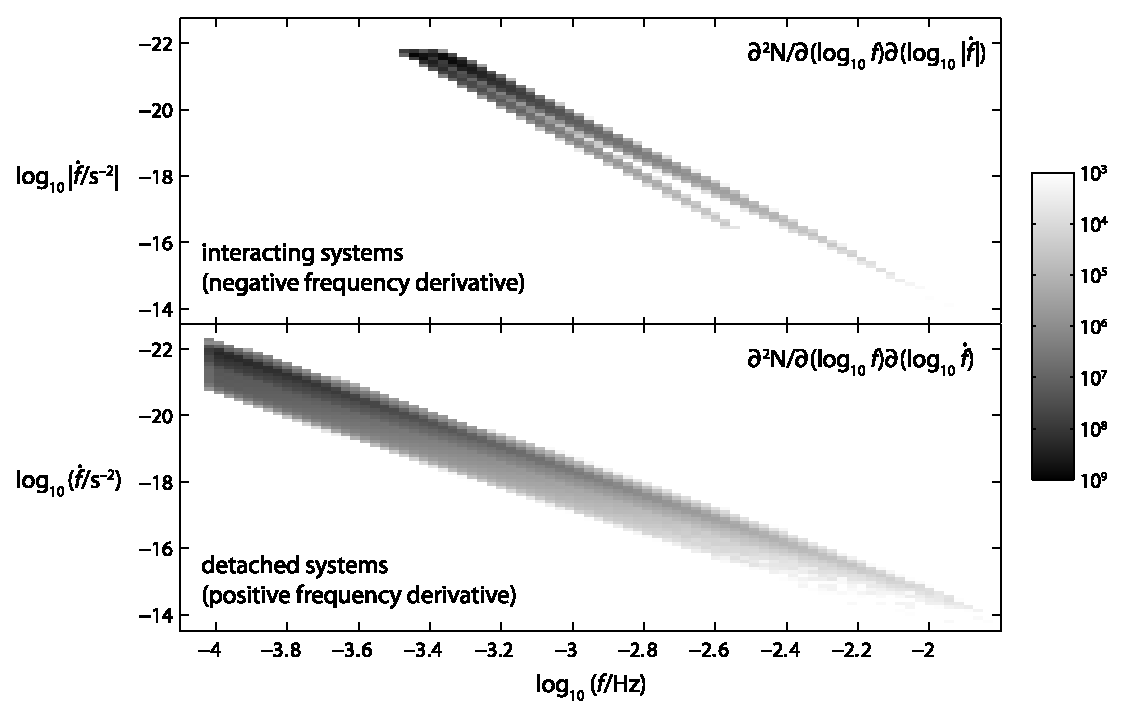
\includegraphics[width=10cm]{densities2b-r.eps}}
\caption{Histogram of the density of Galactic binaries in the Nelemans catalogs, binned by $\log_{10} f$ and $\log_{10} \dot{f}$.\label{fig:binaries}}
\end{figure}

The parameters of each binary in the catalogs are modified by randomly tweaking $f$ by $\pm 1\%$, $A$ by $\pm 10\%$, $\beta$ and $\lambda$ by $\pm 0.5\, {}^\circ$, and by randomly assigning $\psi$, $\iota$, and $\phi_0$ ($\dot{f}$ is computed from the catalog's binary-period derivative and from the tweaked $f$). These random perturbations are large enough to render the original population files useless as answer keys, but small enough to preserve the overall parameter distributions. Binaries with approximate single-Michelson SNR $> 10$ are regarded as ``bright'' and listed in a separate table in the challenge keys. Data set 3.1 includes also 20 verification binaries of known parameters (specified in LISAtools file \url{MLDCwaveforms/Galaxy3/Data/Verification.dat} as rows of $f$, $\dot{f}$, $\beta$, $\lambda$, $A$).

\subsection{Spinning MBH binaries}
\label{sec:ch3mbh}

The spinning-MBH binary GW signals of data set 3.2 are modeled as 2PN circular adiabatic inspirals with uncoupled orbital frequency evolution and spin and orbital precession. No higher-PN harmonics are included. Both phase and orbital
frequency are explicit functions of time (TaylorT3 in classification presented in \cite{DIS}):

\begin{eqnarray}
M\omega &=& \frac1{8}\tau^{-3/8} \left[1 + \left(\frac{743}{2688} + \frac{11}{32}\eta\right)\tau^{-1/4} - 
            \frac3{10}\left(\pi - \frac{\beta}{4}\right)\tau^{-3/8} + 
            \right. \nonumber \\ 
            &+& \left.
            \left(\frac{1855099}{14450688} + 
           \frac{56975}{258048}\eta + \frac{371}{2048}\eta^2 - \frac{3}{64}\sigma\right)\tau^{-1/2}\right]
 \end{eqnarray}
where $\eta = \mu/M$ is symmetric mass ratio and 
\begin{eqnarray}
\tau = \frac{\eta}{5M}(T_c - t),
\end{eqnarray}
\begin{eqnarray}
\beta &=& \frac1{12}\sum_{i=1,2} \left[ 
\chi_i \left(\bL.{\bf \hat{S}_i}\right)\left(113\frac{m_i^2}{M^2} + 75\eta\right)
\right] \\
\sigma &=& -\frac1{48}\eta\chi_1\chi_2\left[ 247(\bSo.\bSt) - 721(\bL.\bSo)(\bL.\bSt)
\right]
\end{eqnarray}
Here $\bL, \; {\bf \hat{S}}_1,\;{\bf \hat{S}}_2$ 
are unit vectors along leading order angular orbital momentum and hole's spins.
The intrinsic orbital phase is 
\begin{eqnarray}
\Phi_{orb} &=& \Phi_C - \frac{\tau^{5/8}}{\eta}\left[ 1 + 
  \left(  \frac{3715}{8064} + \frac{55}{96}\eta \right)\tau^{-1/4}
  - \frac{3}{16}(4\pi - \beta) + \right. \nonumber \\
  & & \left. \left( \frac{9275495}{14450688}+ \frac{284875}{258048}\eta+ \frac{1855}{2048}\eta^2 - \frac{15}{64}\sigma  \right) \tau^{-1/2}
\right]. \label{OrbPhN}
\end{eqnarray}
Due to the spin-orbital coupling the spins and orbital angular momentum are precessing around
total angular momentum, therefor we need to add precessional correction to the orbital 
phase (see \cite{ACST}):

\begin{equation}
\dot{\Phi} = \omega + \frac{(\bL.\hn)[\bL\times \hn]\dot{\bf \hat{L}}_N}{1-(\bL.\hn)^2}
\equiv \omega + \delta\dot{\Phi},\label{totPhi}
\end{equation}
where $\hn$ is direction to the source in SSB. The constant of integration of (\ref{totPhi}),
 $\Phi_C$,  can be redefined so that $\delta\dot{\Phi} = 0$ at $t=0$.  The precession  
 equations for $\bL, \; {\bf \hat{S}}_1,\;{\bf \hat{S}}_2$ are given by eqn. (2.9)-(2.11) in 
 \cite{LangHughes}. As mentioned above we use restricted waveform (only leading order amplitude) and in the source frame (with the phasing formulae above) it takes the following form 
 \begin{eqnarray}
h_{+} &=& -2\frac{\mu}{D}(1 + \cos(i)^2)(M\omega)^{2/3}\cos{2\Phi}\\
h_{\times} &=& 4\frac{\mu}{D}\cos(i)(M\omega)^{2/3}\sin{2\Phi}.
\end{eqnarray}
The inclination angle $i$ is defined by initial position of the orbital momentum and 
by the direction to the source: $\cos{i} = (\bL.\hn)$.
Note that if one uses the approach given in \cite{Kidder}, the amplitudes will be more complicated
and the precession part of the phase at $t=0$ should be $\delta\dot{\Phi}^K = -\gamma^K$,
where superscript $K$ stands for Kidder and 
$$
\gamma^K = \frac{{\bf e}_z \times \bL}{|{\bf e}_z \times \bL|}\frac{\bL\times \hn}
{\sqrt{1 - (\bL.\hn)^2}}.
$$
The end of the inspiral is handled with an exponential taper, as in Challenge 2. The expressions 
for $h_{+}$ and $h_{\times}$ are given in the time varying polarization basis, but to generate the LISA responses it is necessary to re-express it in terms
of fixed polarization tensors. This is achieved through a rotation by the polarization
angle $\psi$:
\begin{equation}
\tan{\psi} = \frac{\cos{\beta}\cos{(\lambda -\phi_L)}\sin{\theta_L} - \cos{\theta_L}\sin{\beta}}
{\sin{\beta}\sin{(\lambda - \phi_L)}}.
\end{equation}
and the waveform in SSB becomes

\begin{eqnarray}
h_{+}^\mathrm{SSB} &=& -h_{+}\cos{2\psi} - h_{\times}\sin{2\psi}\\
h_{\times}^\mathrm{SSB} &=& h_{+}\sin{2\psi} - h_{\times}\cos{2\psi}.
\end{eqnarray}

Masses, SNRs, and times of coalescence are chosen as in Challenge 2 (see also table \ref{table:MLDC3}); the spin magnitudes $S_1/M_1^2$ and $S_2/M_2^2$
are drawn uniformly in $[0,1]$; all the angles (spin directions, initial orbital angular momentum, sky position) are drawn uniformly over spheres. See \url{lisatools/MLDCwaveforms/FastBBH} for the source code.

Dataset 3.2 includes also a Galactic confusion background generated from the same detached-binary population as used in Challenge 3.1 (interacting systems have typically very small chirp masses and are not expected to make a significant contribution), but withholding all binaries with individual SNR $> 5$ relative to instrument noise \textbf{[Neil: is this right?]} The resulting confusion background is described well \textbf{[Neil: is this true?]} by the analytical PSD expression
%
\begin{equation} \fl
S_{X,\mathrm{gal}} = 16 \, x^2 \sin^2 x \, \mathrm{Hz}^{-1} \times \left\{ \begin{array}{l@{}l@{\;}l@{\;}l}
10^{-44.62} &(f/\mathrm{Hz})^{-2.3}  & \mathrm{for} \, f \in [10^{-4}  ,10^{-3}  ] & \mathrm{Hz}, \\ 
10^{-50.92} &(f/\mathrm{Hz})^{-4.4}  & \mathrm{for} \, f \in [10^{-3}  ,10^{-2.7}] & \mathrm{Hz}, \\
10^{-62.8}  &(f/\mathrm{Hz})^{-8.8}  & \mathrm{for} \, f \in [10^{-2.7},10^{-2.4}] & \mathrm{Hz}, \\
10^{-89.68} &(f/\mathrm{Hz})^{-20.0} & \mathrm{for} \, f \in [10^{-2.4},10^{-2.0}] & \mathrm{Hz},
\end{array}\right.
\end{equation}
%
(fractional frequency fluctuations, with $x = 2 \pi f L$, $L \simeq 16.6782$ s), which was derived using a BIC criterion for the resolvability of individual Galactic binaries \cite{Cornish:2007if}, and is used in Challenge 3 (on top of instrument noise) to define the SNRs of GW signals from MBH binaries, EMRIs (Challenge 3.3), and cosmic-string cusps (Challenge 3.4).

\subsection{EMRIs}
\label{sec:ch3emri}

The EMRI waveforms of data set 3.3 are the Barack--Cutler \cite{barackcutler} ``analytic kludges'' used for Challenge 1.3.1--5 and described in \cite[sec.\ 4.5]{mldcgwdaw2}, with the single change in that the number of eccentric-orbit harmonics included in the waveform does not evolve with eccentricity, but is fixed at five (lisaXML parameter \texttt{FixHarmonics}; a value of zero will reproduce the old behavior). See \url{lisatools/MLDCwaveforms/EMRI} for the source code.

\subsection{Cosmic string cusps}
\label{sec:ch3string}

Data set 3.4 contains a number of bursts from cosmic strings, the first of two new GW sources introduced with Challenge 3. Cosmic strings are linear topological defects that may be formed in early Universe at the phase transitions predicted in many elementary-particle and superstring models. Cosmic-string oscillations emit gravitational radiation, with a substantial part of the emission from \emph{cusps}, which can achieve very large Lorentz boosts \cite{cusp1}.
In the limit where the tip of a cusp is moving directly
toward the observer, the observed metric perturbation is a linearly polarized GW with \cite{cusp2}
%
\begin{equation}\label{cusp}
h(t) = A \vert t - t_C \vert^{1/3}, \quad
A \sim \frac{G \mu L^{2/3}}{D_L};
\end{equation}
%
here $t_C$ is the burst's central time of arrival, 
$G$ is Newton's constant, $\mu$ is the string's mass per unit length, $D$
is the luminosity distance to the source, and $L$
is the size of the feature that produces the cusp (e.g., the length of
a cosmic string loop). If the observer's line of sight does not coincide
with the cusp's direction of motion, the waveform becomes a much more
complicated mixture of polarizations~\cite{cusp3}. If the viewing angle $\alpha$ departs
only slightly from zero, the waveform remains dominantly linearly
polarized, and the sharp spike in \eqref{cusp} is rounded
off, introducing an exponential suppression of Fourier-domain power for frequencies above $f_{\rm max} = 2 / (\alpha^3 L)$.

Following the model used by the LIGO Science Collaboration, we define our cusp waveforms
in the Fourier domain according to
%
\begin{equation}
|h_+(f)| = {\cal A} f^{-4/3} \left(1 + (f_{\rm low}/f)^2\right)^{-4}, \quad h_\times = 0,
\end{equation}
%
with $\exp(1 - f/f_\mathrm{max})$ suppression above $f_\mathrm{max}$. The amplitude ${\cal A}$ has dimensions ${\rm Hz}^{1/3}$; $f_{\rm low}$ sets the low-frequency cut-off of what is effectively a fourth-order Butterworth filter, which prevents dynamic-range issues
with the inverse Fourier transforms (for Challenge 3 we set $f_{\rm low} = 1 \times 10^{-5}$ Hz).
The phase of the waveform is set to $\exp \rmi(\pi - 2 \pi f t_C)$ before inverse-Fourier transforming to the time domain. See \url{lisatools/MLDCwaveforms/CosmicStringCusp} for the source code.
% MV 20080328: I checked that Neil's polarization recipe is equivalent to the standard MLDC [see Challenge 2 GWDAW proc, Eq. (5)] if the cusp burst polarization is identified as hp.

\subsection{Stochastic background}
\label{sec:ch3background}

Data set 3.5 contains the second GW source new to Challenge 3: an isotropic, unpolarized, Gaussian and stationary stochastic background. Allen and Romano \cite{stochastic} define a stochastic background as the ``gravitational radiation produced by an extremely large number of weak, independent, and unresolved gravity-wave sources, [...] stochastic in the sense that it can be characterized only statistically.'' Such backgrounds are usually characterized by the dimensionless quantity
%
\begin{equation}
\Omega_\mathrm{gw}(f) = \frac{1}{\rho_\mathrm{crit}} \frac{\rmd \rho_\mathrm{gw}}{\rmd \log f},
\end{equation}
%
with $\rho_\mathrm{gw}$ the energy density in GWs, and $\rho_\mathrm{crit} = 3 c^2 H_0^2 / (8 \pi G)$ the closure energy density of the Universe, and they are idealized as the collective, incoherent radiation of uncorrelated infinitesimal emitters distributed across the sky. If the background is isotropic, unpolarized, Gaussian and stationary, the Fourier amplitude $\tilde{h}_A(f,\hat{\Omega})$ of each emitter (with $A$ indexing the  $+$ and $\times$ polarizations, and $\hat{\Omega}$ the direction on the two sphere) is completely characterized by the power-spectral-density relation \cite{stochastic}
%
\begin{equation} \fl
\big\langle \tilde{h}^*_A(f,\hat{\Omega}) \tilde{h}_{A'}(f',\hat{\Omega}') \big\rangle =
\frac{3 H_0^2}{32 \pi^3}
|f|^{-3} \Omega_\mathrm{gw}(|f|)
\times \delta_{AA'} \delta(f - f') \delta^2(\hat{\Omega},\hat{\Omega}').
\label{eq:pseudosourcepsd}
\end{equation}
%
In Challenge 3, we assume a constant $\Omega_\mathrm{gw}(f)$, as appropriate for the primordial background predicted in many cosmological scenarios. We implement the uncorrelated emitters as a collection of 192 pseudosources distributed at \emph{HEALpix} pixel centers across the sky. HEALpix (the Hierarchical Equal Area isoLatitude Pixelization of spherical surfaces \cite{healpix}) is often used to represent cosmic microwave background data sets; 192 pixels correspond to a twice-refined HEALpix grid with $N_\mathrm{side} = 2^2$.

Each pseudosource consists of uncorrelated pseudorandom processes for $h_+$ and $h_\times$, generated as white noise in the time domain, and filtered to achieve the $f^{-3}$ spectrum of \eqref{eq:pseudosourcepsd}, using the the recursive $1/f^2$ filtering algorithm proposed by Plaszczynski \cite{filtering}, extended to spectral slope $-3$. The algorithm employs a chain of $1/f^2$ infinite--impulse-response filters to reshape the white noise spectrum between minimum and maximum frequencies $f_\mathrm{low}$ and $f_\mathrm{knee}$, set to $10^{-5}$ and $10^{-2}$ Hz in this Challenge (see source code \url{lisatools/MLDCwaveforms/Stochastic.py} for the Synthetic LISA implementation).

The \emph{one-sided} PSD of each single-polarization random process (which represents the finite area of a pixel in the sky) is then given by $S_h(f)/2 = 3 H_0^2/(32 \pi^3) f^{-3} \Omega_\mathrm{gw} \times (4 \pi^2 / 192)$.
In data set 3.5, we define $S^\mathrm{tot}_h = (192 \times 2) S_h$ and we set it so that, in the TDI observables, the GW background is a few times stronger than LISA's secondary instrument noise. Namely, 
%
\begin{equation}
S^\mathrm{tot}_h(f) = 0.7\mbox{--}1.3 \times 10^{-47} (f/\mathrm{Hz})^{-3} \, \mathrm{Hz}^{-1}
\end{equation}
%
(taking $H_0 = 70 \, \mathrm{km} / \mathrm{s} / \mathrm{Mpc}$, this corresponds to $\Omega_\mathrm{gw}=8.95\times 10^{-12}\mbox{--}1.66\times 10^{-11}$). \textbf{[Check the 1/2 for the one-sided spectrum.]}

One of the more promising approaches to detect GW backgrounds with LISA relies on estimating instrument noise levels by way of symmetrized TDI observables that is insensitive to GWs at low frequencies in the LISA band \cite{zetapaper}. For realistic LISA orbits, however, the low-frequency behavior of such observables becomes more complicated than discussed in the literature. To simplify the initial investigation of the background-detection problem in data set 3.5, we have therefore approximated 
LISA as a rigidly rotating triangle with equal and constant armlengths (i.e., Synthetic LISA's \url{CircularRotating}).

\section{Conclusion}

We are very excited about the outcome of the first two MLDCs, which have given a convincing demonstration that a significant portion of the LISA science objectives could already be achieved with techniques that are currently in hand. Most of the research groups that participated in Challenge 1 have successfully made the transition to the greater complexity of Challenge 2. Challenge 3 (with data sets released in Jan 2008 and results due in Dec 2008) will continue to move in the direction of more realistic signals, featuring chirping Galactic binaries and precessing binaries of spinning MBHs. It will also include two new classes of signals: an isotropic primordial GW background and bursts from the cusps of cosmic strings. In addition, Challenge 1B took place between July and Dec 2007. This was a repeat of Challenge 1, conceived to provide a softer entry point for research groups new to the MLDCs. Ten collaborations (including five new institutions) participated, demonstrating increasing sophistication and proficiency in a range of LISA data-analysis techniques.

Furthermore, the MLDC conventions, file formats, and software tools (see \url{lisatools.googlecode.com}) have matured to the point where interested parties can use them to generate a variety of data sets. This enables a wealth of interesting side investigations, such as the studies of the LISA science reach that are now being undertaken by the LISA Science Team. To obtain more information and to participate in the MLDCs, see the official MLDC website (\url{astrogravs.nasa.gov/docs/mldc}) and the task force wiki (\url{www.tapir.caltech.edu/listwg1b}).
\textbf{[These two paragraphs are verbatim from the MLDC-2 report. Need to shorten, rephrase, add more about results.]}

\ack

MV: the LISA Mission Science Office and by JPL's HRDF.
CC's, JC's and MV's work was carried out at the Jet Propulsion Laboratory, California Institute of Technology, under contract with the National Aeronautics and Space Administration.
SB's and EP's work was supported by the Deutsches Zentrum f\"ur Luft- und Raumfahrt.
JG thanks the Royal Society for support and the Albert Einstein
Institute for hospitality and support while part of this work was
being completed. IM was partially supported by NASA ATP Grant
NNX07AH22G to Northwestern University. LW's work is supported by the
Alexander von Humboldt Foundation's Sofja Kovalevskaja Programme
funded by the German Federal Ministry of Education and Research.
MT acknowledges the support of the Spanish Ministerio de Eduaci\'on y
Ciencia Research projects FPA-2007-60220, CSD207-00042 and the Govern
de les Illes Balears, Conselleria d'Economia, Hisenda i Innovaci\'o.

% \appendix

% \section{SNR and cross-spectra}

\section*{References}

\begin{thebibliography}{99}
%
\bibitem{lisa} Bender P, Danzmann P and the LISA Study Team 1998 ``Laser Interferometer Space Antenna for the Detection of Gravitational Waves, Pre-Phase A Report'' \textbf{MPQ 233} (Garching: Max-Planck-Instit\"ut f\"ur Quantenoptik) 
%
\bibitem{mldclisasymp} Arnaud K A et al. (the MLDC Task Force) 2006 \textit{Laser Interferometer Space Antenna: 6th International LISA Symp. (Greenbelt, MD, 19--23 Jun 2006)} ed Merkowitz S M and Livas J C (Melville, NY: AIP) p 619; \textit{ibid.} p 625 (long version with lisaXML description: \textit{Preprint} gr-qc/0609106)
%
\bibitem{mldcgwdaw1} Arnaud K A et al. (the MLDC Task Force and Challenge 1 participants) 2007 \textit{Class. Quant. Grav.} \textbf{24} S529
%
\bibitem{barackcutler} Barack L and Cutler C 2004 \textit{Phys. Rev.} D \textbf{69} 082005
%
\bibitem{mldcgwdaw2} Arnaud K A et al. (the MLDC Task Force) 2007 \textit{Class. Quant. Grav.} \textbf{24} S551
%
\bibitem{mldcamaldi2} Babak S  et al. (the MLDC Task Force and the Challenge 2 Participants) 2007 \textit{Preprint}  arXiv:0711.2667
%
\bibitem{JKS98}
P.\ Jaranowski, A.\ Kr\'olak, and B.\ F.\ Schutz, Phys.\ Rev.\ D
{\textbf 58}, 063001 (1998).
%
\bibitem{KTV04} A. Kr\'olak, M. Tinto, and M. Vallisneri, {\it Phys. Rev. D}, {\bf 70},
022003 (2004).
%
\bibitem{prixwhelan} Prix R and Whelan J T 2007 \textit{Class. Quant. Grav.} \textbf{24} S565; \textit{Poster} \url{www.ligo.caltech.edu/docs/G/G070462-00.pdf}
%
\bibitem{cornishporter} Cornish N J and Porter E K 2007 \textit{Class. Quantum Grav.} \textbf{24} 5729--5755
%
\bibitem{brown} Brown D A, Crowder J, Cutler C, Mandel I and Vallisneri M 2007 \textit{Class. Quant. Grav.} \textbf{24} S595
%
\bibitem{VCT} Vallisneri M, Crowder J and Tinto M 2007 ``Sensitivity and parameter-estimation precision for alternate LISA configurations'' \textit{Preprint} arxiv.org/0710.4369 
%
\bibitem{gair} Gair J R, Mandel I and Wen L 2007 Proc. 7th Amaldi Conf. on Gravitational Waves (Sydney, 8--14 July 2007), submitted. \textit{Preprint} arXiv:0710.5250
%
\bibitem{Nelemans:2001hp} G. Nelemans, L. R. Yungelson \& S. F. Portegies Zwart, A\&A {\bf 375}, 890 (2001).
%
\bibitem{Nelemans:2003ha} G. Nelemans, L. R. Yungelson \& S. F. Portegies Zwart, Mon. Not. Roy. Astron. Soc.
{\bf 349} 181, (2004).
%
\bibitem{Cornish:2007if} N.~J.~Cornish and T.~B.~Littenberg, Phys.\ Rev.\ D {\bf 76}, 083006 (2007).
%
\bibitem{Roelofs:2007rn} G.~H.~A.~Roelofs, G.~Nelemans and P.~J.~Groot,
``The population of AM CVn stars from the Sloan Digital Sky Survey,''
arXiv:0709.2951 [astro-ph].
%
\bibitem{cusp1} T. Damour and A. Vilenkin, Phys. Rev. Lett. {\bf 85}, 3761 (2000).
%
\bibitem{cusp2} X. Siemens, J. Creighton, I. Maor, S. Ray Majumder,
K. Cannon, and J. Read, Phys. Rev. D {\bf 73} 105001 (2006).
%
\bibitem{cusp3} X. Siemens and K. D. Olum, Phys. Rev. D {\bf 68}, 085017 (2003).
%
\bibitem{stochastic} B. Allen and J. D. Romano, Phys. Rev. D {\bf 59}, 102001 (1999).
%
\bibitem{healpix} K. M. G\'orski et al., Astrophys. J. {\bf 622}, 759 (2005).
%
\bibitem{filtering} S. Plaszczynski, Fluctuation and Noise Letters {\bf 7}, R1 (2007) [arXiv:astro-ph/0510081].
%
\bibitem{zetapaper} M. Tinto, J. W. Armstrong and F. B. Estabrook, Phys. Rev. D 63, 021101 (2000).
%
\bibitem{DIS} T. Damour, B. Iyer and B. Sathyaprakash, Phys. Rev. D {\bf 63}, 044023 (2001).
%
\bibitem{ACST} T. A. Apostolatos, C. Cutler, G. J. Sussman and K. S. Thorne, Phys. Rev. D {\bf 49},
6274 (1994)
%
\bibitem{LangHughes} R. N. Lang and S. A. Hughes, Phys. Rev. D {\bf 74}, 122001 (2006) 
%
\bibitem{Kidder} L. Kidder, Phys. Rev. D {\bf 52}  821 (1995)
%
\bibitem{gmw} J. R. Gair, I. Mandel and L. Wen
``Improved time-frequency analysis of extreme-mass-ratio inspiral signals in mock LISA data,'' proceedings of GWDAW-12, Dec 13--16 2007, Cambridge MA.
%
\bibitem{tvv} M. Trias, A. Vecchio and J. Veitch,
``Markov Chain Monte Carlo searches for Galactic binaries in MLDC-1B data sets,'' proceedings of GWDAW-12, Dec 13--16 2007, Cambridge MA.
%
\bibitem{lisacode} A. Petiteau, G. Auger, H. Halloin, O. Jeannin, E. Plagnol, S. Pireaux, T. Regimbeau and J.-Y. Vinet, Phys. Rev. D {\bf 77}, 023002 (2008).
%
\bibitem{lisasimulator} Cornish N J and Rubbo L J 2003 \emph{Phys. Rev. D} \textbf{67} 022001; erratum-ibid. 029905; LISA Simulator website, \url{www.physics.montana.edu/lisa}; the LISA Simulator is now automatically downloaded as part of the LISAtools installation (see \url{lisatools.googlecode.com})
%
\bibitem{synthlisa} Vallisneri M 2005 \emph{Phys. Rev. D} \textbf{71}; Synthetic LISA website, \url{www.vallis.org/syntheticlisa}; Synthetic LISA is now automatically downloaded as part of the LISAtools installation (see \url{lisatools.googlecode.com})
%
\bibitem{cardiffmbh} I. Harry, S. Fairhurst, B. S. Sathyaprakash, ``A Search for Super Massive Black Hole Coalescences in the Mock LISA Data Challenges,'' proceedings of GWDAW-12, Dec 13--16 2007, Cambridge MA.
%
\end{thebibliography}
\end{document}




